\chapter{Modelos de comportamiento colectivo} \label{cap2}

En este capítulo se explica detalladamente el significado del término swarming y su impacto en diferentes aspectos de la ciencia. Es innegable que el movimiento que presentan algunas bandadas de pájaros es hipnótico, al igual que es sorprendente cómo algunos insectos como las abejas se organizan para construir los paneles y recolectar la miel, o las hormigas que lo hacen para conseguir recolectar su comida. Todo estos comportamientos que nos ofrece la naturaleza se llevan estudiando desde 3 décadas intentando modelarlos a través de las matemáticas y aplicarlos a través de la tecnología.

\section{Comportamiento colectivo} \label{s2_1}
En los últimos años se ha incrementado considerablemente las investigaciones sobre esta nueva forma de inteligencia: la inteligencia de enjambre, o \textit{Swarm Intelligence} (SI por sus siglas en inglés). Pero, ¿de dónde viene el interés de esta nueva corriente de investigación y en qué se basa? En esta sección se abordará la base biológica del estudio haciendo un repaso de las formaciones que más se han utilizado para el estudio del \textit{swarming} en la ciencia.

Para conocer el contexto y la magnitud del tema que se va a abordar, el estudio del movimiento grupal auto-organizado no se limita únicamente a criaturas relativamente simples como enjambres de insectos o bancos de peces, si no que puede abarcar todo el espectro de la taxonomía de los seres vivos, desde bacterias y elemento moleculares simples \cite{nicolis1977selfOrg} hasta animales inteligentes como los seres humanos; lo que diferencia estos estudios es la complejidad de cada uno y por tanto, de sus acciones. Uno de los ejemplos más desastrosos y complejos del movimiento colectivo tiene que ver con los seres humanos y las estampidas inducidas por el pánico, que a menudo conducen a la muerte de personas aplastadas y pisoteadas. A continuación se abordarán 3 enfoques diferentes a la hora de estudiar la auto-organización de ciertos seres vivos.

Aunque los próximos estudios que se van a mencionar están todos englobados bajo la rama de comportamiento colectivo en animales sociales, cabe destacar que para una mejor comprensión de todos ellos, se pueden diferenciar dos tipos dependiendo de la finalidad de su organización. En primer lugar existen aquellos en los que la finalidad de la auto-organización del grupo se hace con fines meramente productivos como por ejemplo recolectar comida o construir nidos. Por otro lado, pueden diferenciarse también los que se auto-organizan para mejorar el movimiento y la dinámica del grupo, como por ejemplo, mejorar la aerodinámica o disminuir la dispersión del grupo. En las próximas dos secciones se va a profundizar en cada uno de ellos.

\subsection{Comportamiento colectivo en animales sociales}\label{s2_1_1}
La observación de insectos sociales que viven en colonias como las hormigas, las abejas, las avispas y las termitas han servido de fuente a muchas investigaciones debido a la alta capacidad de organización e integración de cada individuo para realizar tareas más complejas en las que intervienen todo el grupo. Muchas actividades colectivas realizadas por este tipo de insectos dan como resultado patrones espacio-temporales complejos. Los etólogos a menudo tienen la tentación de asumir que tales patrones complejos a nivel de colonia solo pueden ser generados por individuos complejos, es decir, por individuos que pueden tener en cuenta numerosos parámetros para modular sus comportamientos.  Las teorías sobre auto-organización, por su parte, pueden extenderse a los sistemas etiológicos, particularmente a las inserciones sociales, para mostrar que los comportamientos colectivos complejos pueden surgir de interacciones entre individuos que exhiben comportamientos simples. En esta línea se pueden leer referencias como esta de Robinson \cite{robinson1992regulation}.

En el caso de las hormigas se puede ver un ejemplo de cómo se organizan en grupos especializados dependiendo de su edad o su morfología. La especie de las hormigas cortadoras (\textit{Atta}) corta hojas de plantas y árboles mientras que las trabajadoras transportan esas hojas hasta sus sitios de forraje a cientos de metros donde se dan las condiciones perfectas para la formación de hongos, creando a su vez caminos óptimos hacia, desde y entre estos nidos \cite{CherrettAtta}.

Las hormigas tejedoras (\textit{Oecophylla}), forman grandes cadenas con sus propios cuerpos permitiéndoles de esta manera cruzar espacios amplios entre hojas como se muestra en la figura \ref{fig:hormiga-tejedora-a}. Estas formaciones sirven tanto para que las trabajadoras crucen entre hojas, como para que las propias tejedoras puedan reunir suficiente fuerza como para juntar ambas y conectarlas con un hilo de seda. Este comportamiento lo explican  \citeauthor*{bonabeau1999swarm} en \cite{bonabeau1999swarm} y se muestra en este documento en la figura \ref{fig:hormiga-tejedora-b}. Se cree que esta división del trabajo entre los compañeros de nido, según la cual las actividades se realizan simultáneamente por grupos de individuos especializados, es más eficiente que si las tareas fueran realizadas de forma secuencial por individuos no especializados. Estas ideas se reflejan originalmente en los artículos \cite{jeanne1986evolution,robinson1992regulation}.

\begin{figure}[!ht]
\centering
    \subcaptionbox{Puente\label{fig:hormiga-tejedora-a}}{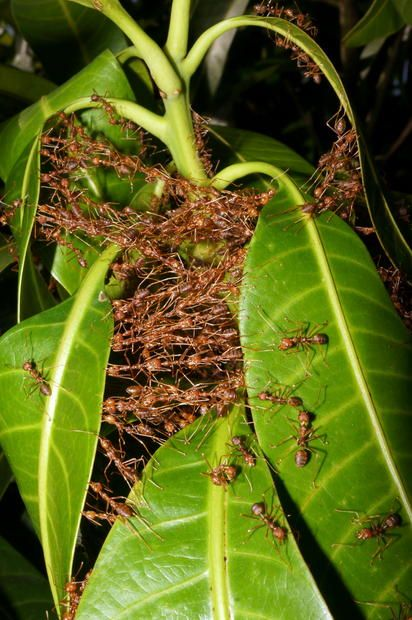
\includegraphics[height=40mm]{fig/cap02/hormiga_tejedora.jpg}}\hspace{3cm}
    \subcaptionbox{Tejiendo dos hojas\label{fig:hormiga-tejedora-b}}{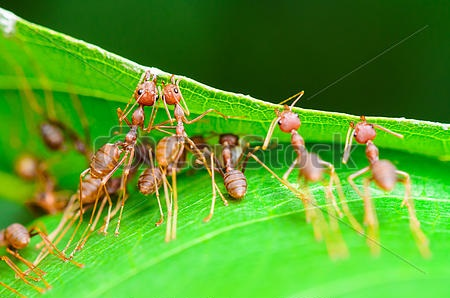
\includegraphics[height=40mm]{fig/cap02/oecophylla-tejiendo.jpg}}
\caption{Hormiga tejedora (\textit{Oecophylla})} 
\label{fig:Figura_HormigaTejedora}
\end{figure}

Las abejas por su parte, organizan sus colmenas en paralelo formando cadenas que inducen a un aumento de temperatura permitiendo así que sea más fácil moldearlas, como es el caso de la especie (\textit{Apis mellifica}) tal y como se puede observar en la figura \ref{fig:Figura_EnjambreAbeja}. En ciertos momentos la colonia se divide de tal forma que la abeja reina y la mitad aproximadamente de las trabajadoras abandonan la colmena formando un grupo en una rama cercana. Las exploradoras por su parte, exploran cuidadosamente los sitios potenciales de anidación pudiendo durar este proceso de selección varios días.

\begin{figure}[!ht]
\centering
    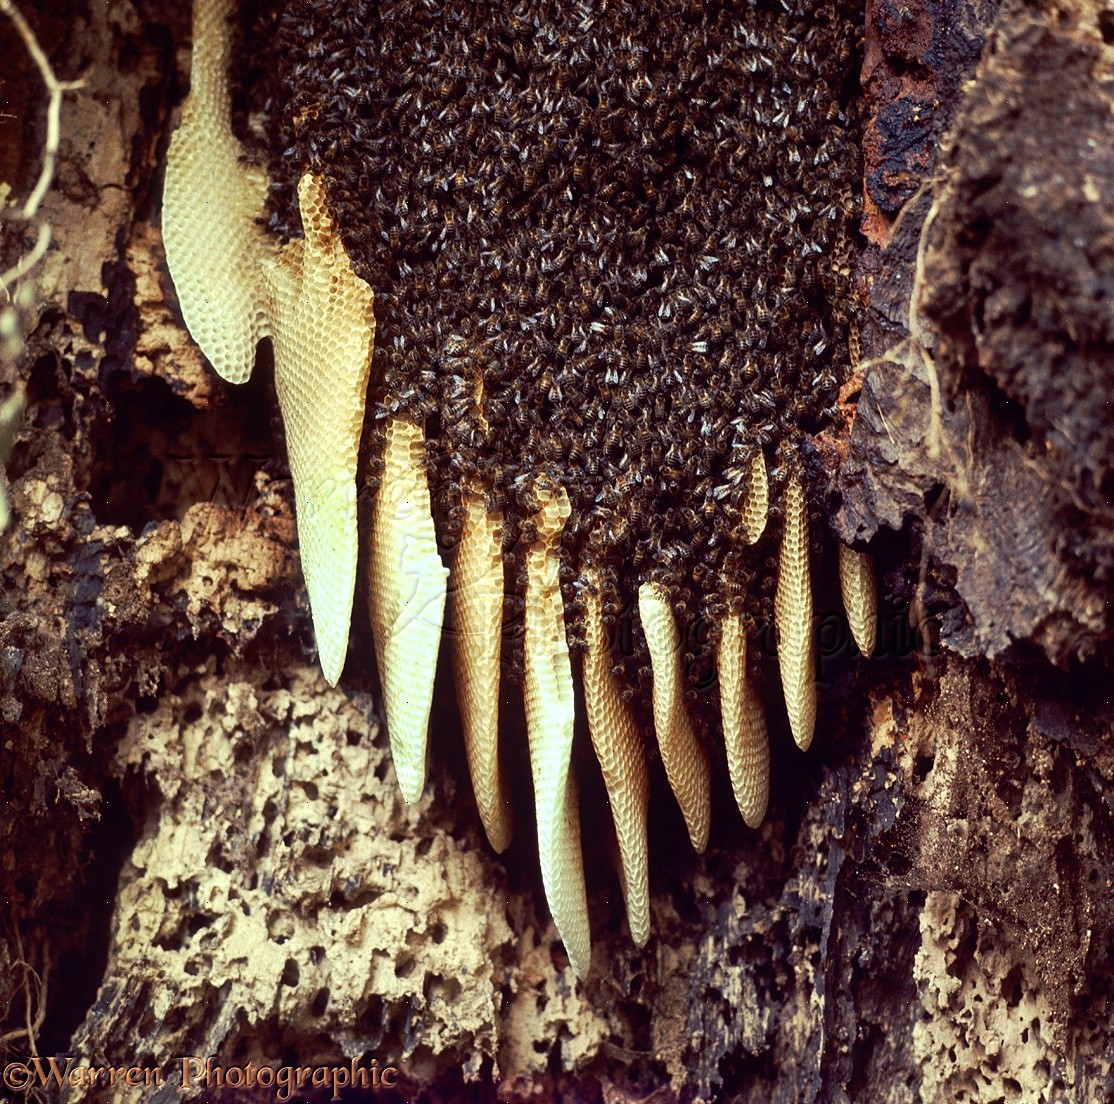
\includegraphics[height=6cm]{fig/cap02/Honey-Bee-comb.jpg}
    \caption{Enjambre de abejas \textit{Apis mellifica}}
    \label{fig:Figura_EnjambreAbeja}
\end{figure}

Estos tipos anteriormente descritos de comportamiento en insectos sociales son referentes a la organización de las tareas del grupo, en función de las características de cada individuo con una finalidad clara de mejorar la productividad. Se pueden leer más ejemplos de insectos sociales en las referencias \cite{csahin2004swarm,robinson1992regulation}. 

Existe otro tipo de comportamiento colectivo, que hace referencia a la dinámica del grupo que se observa en bandadas de pájaros, manadas de animales o bancos de peces, entre otros. Éste hace referencia al comportamiento individual de cada animal que les permita coordinar sus movimientos en relación a los demás integrantes del grupo. Existen numerosos artículos y estudios sobre el comportamiento de los peces y la formación de bancos de peces (\textit{Schooling})\footnote{Según I. Aoki: ``Resultado de las interacciones en las que un individuo controla su movimiento en relación con los vecinos y, al mismo tiempo, influye en estos vecinos"} dependiendo de diferentes factores externos. Una pequeña muestra de artículos relacionados con esta rama de estudio son \cite{aoki1982simulation, Aoki1984experimental,hall1910hidden,partridge1980sensory,partridge1980three,Pitcher963blindfish,youseff2008parallel}. 

Aoki, en su artículo \cite{aoki1982simulation} estudia el comportamiento de cada individuo del banco en función de la distancia del vecino más cercano. Para ello, basó sus estudios en un principio de la organización de los bancos de peces que estableció Edward T. Hall \cite{hall1910hidden}, según el cual el comportamiento depende tanto de la distancia personal como de la distancia social y se encontró con que los movimientos grupales podrían ocurrir a pesar de que cada individuo careciese de conocimiento del movimiento de todo el banco y en ausencia de un líder consistente. Esto podía ocurrir si individualmente llevaban a cabo tanto un movimiento de aproximación que permitiera la agregación como un movimiento de orientación paralela para que el banco mantuviera la cohesión.

Atendiendo en esta ocasión al comportamiento de las aves, estas bandadas naturales parecen basar su movimiento en dos comportamientos opuestos y equilibrados: el deseo de permanecer cerca de la bandada y el deseo de evitar colisiones entre cada ave. Pero aunque la razón por la que desean evitar colisiones parece evidente, ¿por qué deciden permanecer unidos a pesar de que sería más fácil el vuelo por separado?. El impulso básico de las aves para unirse a una bandada es el resultado de la presión evolutiva de varios factores como la protección contra los depredadores, una búsqueda más fácil de alimentos aumentando el patrón de búsqueda o las ventajas para las actividades sociales y de apareamiento. Esto lo trata \citeauthor{reynolds1987flocks} en su artículo \cite{reynolds1987flocks} y más adelante se tratará con más profundidad en este trabajo.

\begin{figure}[!ht]
    \centering
    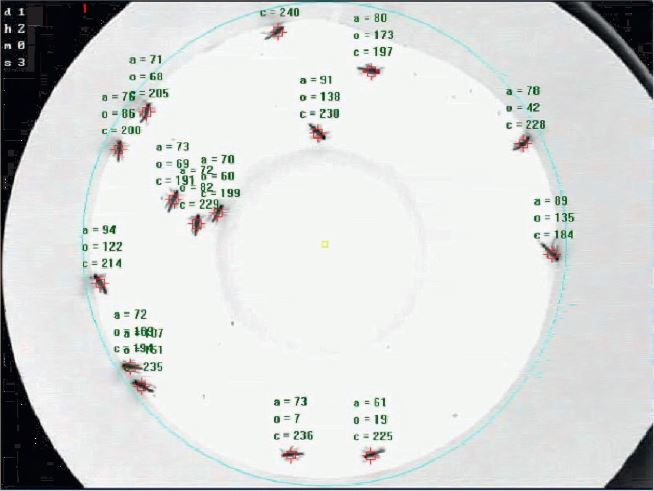
\includegraphics[height=8cm]{fig/cap02/Locusts.JPG}
    \caption{Langostas en el Sombrero Mexicano monitorizadas con el software que utilizó \citeauthor{buhl2006disorder} en sus estudios}
    \label{fig:locust_mexican_hat}
\end{figure}

\citeauthor{buhl2006disorder}\cite{buhl2006disorder} hicieron un estudio sobre las langostas en el que observaron que las juveniles se agrupaban fácilmente en bandas de marcha altamente coordinadas en condiciones de laboratorio, cuando las colocaron en un terrario en forma de `sombrero mexicano'. Los individuos seleccionaron colectivamente una dirección de movimiento en sentido horario o en sentido antihorario aleatoriamente y mantuvieron esto durante períodos prolongados. El movimiento de las langostas se registró durante ocho horas y los datos resultantes se procesaron utilizando el software de seguimiento para calcular la posición y orientación de cada langosta (véase la figura \ref{fig:locust_mexican_hat}). \citeauthor{buhl2006disorder} llegaron a la conclusión de que este comportamiento dependía en gran medida de la densidad de población en el sombrero. A mayor densidad, mayor era la alineación de los movimientos en el grupo.


Aunque el efecto de agregación en animales es obvio y claramente visible al ojo humano (peces, aves, insectos...) el análisis heurístico únicamente basado en lo que vemos no es suficiente para responder a la pregunta fundamental de cómo y por qué ocurre esto. Parrish analiza en conjunto los estudios anteriores en busca de similitudes y diferencias entre los diferentes algoritmos, identificando la relación entre el comportamiento individual de cada individuo y el del conjunto del grupo en \cite{parrish2002self}. 

En un principio, Parrish identifica dos maneras de ver la integración de los animales en un grupo; por una parte, existen animales territoriales con poca necesidad de participar en la transferencia de información y sin necesidad de estructura grupal y por otra, la que interesa desde el punto de vista del \textit{Swarming}, se encuentran las asociaciones altamente integradas a largo plazo. En las segundas tienen lugar altas tasas de intercambio de información, están compuestas por individuos que se conocen y están relacionados con otros miembros, siendo evolutivamente más beneficiosos ya que el contacto sensorial entre individuos es el reflejo de las condiciones ambientales o morfologías de los organismos.

Los estudios que se han hecho hasta el momento han sido en condiciones muy artificiales, generalmente con un número reducido de individuos debido a la dificultad de recoger datos fiables. Por ejemplo, en el caso de la observación de un banco de peces, es fácil entender la complejidad a la que se exponen los investigadores debido a que por una parte, se realizan en un medio acuático y por otra parte, hay peces más profundos en el mismo banco que no se ven desde la superficie e intervienen igualmente en el movimiento colectivo. Por tanto, mientras las técnicas de observación de estos animales no avancen, es difícil obtener una relación entre el comportamiento de un pez y el grupo. Parrish recoge los datos de los estudios anteriores más relevantes para compararlos entre ellos, aunque cada uno contenga datos relativamente diferentes. Tras la comparación se puede observar que no siempre se consigue el consenso en la dirección de los peces del banco. En la tabla \ref{tab:tablaRaynolds} se recogen algunos de todos los que Parrish compara en su artículo.

\begin{center}
\begin{spacing}{0.5}
    \small{
    \begin{table}[t]%[h!]
        \begin{tabularx}{1\textwidth}{>{\raggedright\arraybackslash}X >{\raggedright\arraybackslash}X >{\raggedright\arraybackslash}X >{\raggedright\arraybackslash}X >{\raggedright\arraybackslash}X} 
            \hline
            Referencia & Tamaño de la población & Orientación de partida & Velocidad & ¿Consenso?\\  
            \hline\hline
            Aoki (1982,1984) & 8,32 & Posición aleatoria y orientación dentro de área delimitada & Aleatoria & Sí\\ 
            \hline
            Warburton y Lazarus(1991) & 2-9 & Rejilla cuadrada & Sin especificar & No\\
            \hline
            Huth y Wissel (1990-92-94)& 8 & Posición aleatoria y orientación en área fija & Aleatoria & Sí\\
            \hline
            Reuter y Breckling (1994) & 10, 20, 30, 40, 50 & Posición aleatoria y orientación dentro de área delimitada & Difusa & Sí\\
            \hline
            Romey (1996) & 2-10 & Posición aleatoria y orientación dentro de área delimitada & Constante & No\\
            \hline
            Vab{\o} y N\o ttestad (1997) & 900 & Posición aleatoria y orientación dentro de área fija y delimitada & Constante & No\\ 
            \hline
            Stocker (1999) & 12, 64 & Posición aleatoria y orientación dentro de área delimitada & Constante & Sí\\ 
            \hline
            
        \end{tabularx}
        \caption{Tabla de Reynolds comparativa de los diferentes estudios}
        \label{tab:tablaRaynolds}
    \end{table}
    }
\end{spacing}
\end{center}

\newpage
\clearpage

\subsection{Auto-organización en la robótica} \label{s2_1_2}

La estructura organizativa que tienen los animales vistos hasta ahora tiene un gran beneficio si lo aplicamos a los enjambres de robots \footnote{\textit{Swarm robotics}: La robótica de enjambre es el estudio del diseño de un gran número de agentes físicos relativamente simples de modo que el comportamiento colectivo deseado surja de las interacciones locales entre los propios agentes y entre los agentes y el medio ambiente.\cite{csahin2004swarm}}. Hoy en día cada vez son más las tareas que tienden a automatizarse y para muchas de ellas son necesarios un grupo de robots. Además, las propiedades que caracterizan un sistema auto-organizado, como la escalabilidad, la flexibilidad y la robustez, también son muy deseables para un enjambre de robots autónomos. Es debido a esta creciente importancia que este enfoque merece ser explicado. En \cite{christian2008swarm} los autores introducen un estudio de este concepto antes de presentamos una breve revisión de la investigación en robótica de enjambres a lo largo de cuatro ejes: diseño, modelado y análisis, robots y problemas.

Son las tres características mencionadas anteriormente las que usa como nexo de unión entre la auto-organización aplicada a la biología y a la robótica: 

\begin{itemize}
    \item \textbf{Robustez}: en los enjambres la pérdida de un individuo puede ser inmediatamente compensada por otro, la coordinación está descentralizada y, por lo tanto, es poco probable que la destrucción de una parte particular del enjambre detenga su operación, la simplicidad de los individuos los hace menos propensos al fracaso y la percepción sensorial se distribuye y por tanto, el sistema es robusto frente a las perturbaciones locales del entorno.
    \item \textbf{Flexibilidad}: los individuos de un enjambre deben ser capaces de coordinar sus comportamientos para abordar tareas de diferente naturaleza.
    \item \textbf{Escalabilidad}: debe poder operar en una amplia gama de tamaños de grupo y apoyar a una gran cantidad de individuos sin afectar considerablemente el rendimiento.
\end{itemize}

A estas características los autores añaden otras que debe tener el enjambre como tener una forma y masa y ser capaces de interactuar físicamente con su entorno, ser idénticos al menos en la manera de interactuar, ser capaces de realizar la tarea con la mayor simpleza posible y tener habilidades de interacción local. Además cabe destacar que dos de los principales mecanismos de coordinación que funcionan en los sistemas naturales son válidos para los sistemas robóticos y son la auto-organización y la estigmergia \footnote{\textit{Estigmergia}: en biología, se refiere a la capacidad que tienen algunos sistemas descentralizados de contribución a través del medio que los rodea} (se puede leer más sobre este término en \cite{estigmergia1} y \cite{estigmergia2}). 

Una vez sentadas las bases teóricas sobre las características que deben tener un enjambre de robots, \citeauthor{christian2008swarm} recorren lo que ellos consideran son las líneas de investigación para poder desarrollarlo. 

En cuanto al diseño, agrupa los estudios en en función de si lo que se busca es que cumpla una funcionalidad o \textit{ad-hoc} o que se diseñe en base a unos principios. Un diseño ad-hoc asume implícitamente que el enjambre el grupo de robots va a tener un comportamiento similar a los insectos o animales utilizados como inspiración. En el diseño basado en principios en lugar de diseñar un comportamiento específico a nivel de enjambre, se utiliza una metodología general a través de la cual se pueden usar los comportamientos deseados a nivel de enjambre para construir los comportamientos individuales necesarios.

Otra linea de investigación es el modelado y análisis, para lo cual divide 3 tipos diferentes de modelado. El primero, basado en sensores, es utilizado principalmente para construir simuladores realistas de sistemas robóticos y nos permite realizar experimentos en simulación y así obtener resultados que se aproximan en mayor medida con los obtenidos de los robots físicos. En segundo lugar, existe el modelado microscópico que tiene en cuenta las características del entorno, la forma física y el control del comportamiento de los robots de tal manera que a la vez que simula las interacciones individuales dentro del sistema, también es capaz de adaptar los estados individuales en el tiempo. Por último, el modelado macroscópico simula el comportamiento de unas cantidades medias que representan el estado del sistema. Este último es común en física y química y es suficiente con resolverlos solo una vez para obtener el estado estacionario del modelo.

Otra de las principales líneas de investigación ha sido el desarrollo de enjambres de robots físicos, ya que la construcción de un sistema robótico requiere más que reunir una cantidad de copias de una plataforma robótica genérica. Todos los estudios con este fin se han centrado en el desarrollo de robots móviles que tienen como objetivo proporcionar una plataforma de investigación y no están destinados a la operación en el mundo real. A los ya mencionados con anterioridad existen una serie de requisitos adicionales que deben tener estos sistemas físicos desde el punto de vista de los investigadores que tienen que ver con la detección y señalización de los propios robots, la comunicación, la interacción física entre ellos y con el entorno, la fuente de energía de la que disponen y cómo la utilizan, el costo de producción y de puesta en marcha, el tamaño o tener simuladores.

Esta última aplicación de enjambres de robots, aún se encuentra en una fase muy inicial de desarrollo pero sin lugar a duda, es la que presenta el mayor potencial de aplicación para el futuro de la robótica.


\section{Modelos matemáticos} \label{s2_2}
Para comprender el contexto de los modelos matemáticos que estudian el comportamiento colectivo, 

Los modelos matemáticos que estudian el comportamiento colectivo encuentran una fuerte base en los modelos clásicos que han servido históricamente para estudiar el crecimiento de conjuntos de poblaciones.

\subsection{Modelos clásicos poblacionales} \label{s2_2_1}
En este apartado, hay 3 modelos clásicos que requieren una breve explicación:

\subsubsection{Modelo de Malthus}
En su artículo \cite{malthus1846ensayo} quería demostrar que nuestro crecimiento es insostenible y acabaría desembocando en una pauperización y en una economía de subsistencia, si no directamente en la extinción. Malthus utiliza el modelo de crecimiento exponencial del Carbono 14 para emular el crecimiento poblacional, es decir, cada año la población aumenta o disminuye un cierto tanto por uno $p$ respecto a lo que había el año anterior según la siguiente fórmula:

\begin{equation}
    N_{k} = N_0\cdot C_k \quad \textrm{donde} \quad C = (1+\Delta tR_0)
\end{equation}

\noindent que si lo pasamos al modelo continuo haciendo tender $\Delta t -> 0$ queda:

\begin{equation}
    N'(t) = C \cdot N(t) => N(t) = N_0 \cdot e^{Ct}
\end{equation}

\subsubsection{Modelo Logístico}
Tras leer el ensayo de Malthus, Pierre-Fran\c{c}ois Verhulst \cite[Cap.~37,38]{haberman1998mathematical} publica un nuevo modelo basándose en el de su predecesor, pero añadiendo que la tasa de reproducción es proporcional tanto a la población existente como, además, a la cantidad de recursos disponibles, asumiendo así que existe un punto de saturación el cual significa que si la población crece mucho, entonces te quedas sin recursos para abastecerla y por tanto deja de crecer. Según esto, el modelo Logístico discreto que propone Verhulst queda de la siguiente forma:

\begin{equation}
    \displaystyle{\frac{\Delta N}{\Delta t} = (C_1 \cdot N_k) \cdot (C_2 \cdot (1-N_k)}
\end{equation}

\noindent que agrupando algunas de las constantes y re-escalando la unidad de medida del número de individuos se obtiene:

\begin{equation}
    N_{k+1} = C \cdot N_k \cdot (1 - N_k)
\end{equation}

\noindent cuya solución del modelo continuo quedaría:

\begin{equation}
    \displaystyle{N(t) = \frac{\frac{a}{b}}{1+(\frac{a-bN_0}{bN_0})e^{-at}}} 
\end{equation}

Una evolución de este modelo sería el que propone Lotka Volterra \cite[Cap.~43]{haberman1998mathematical} que lo aplica a dos sistemas coexistentes, de los cuales uno es el sistema depredador y otro es el sistema presa estando estrechamente relacionado la evolución de ambos.


\subsection{Modelo de Keller-Segel} \label{s_2_2_2}
Otro modelo matemático de importancia es el presentado por Evelyn Fox Keller y Lee A. Segel \cite{keller1970initiation, keller1971model, keller1971traveling}, que estudian el comportamiento de insectos cuyos comportamientos y movimientos los llevan a cabo de acuerdo a unos gradientes de sustancias químicas. Este modelo ha sido muy utilizado en diversos ensayos, algunos de los cuales más importantes pueden leerse en las referencias \cite{calvez2008parabolic, blanchet2008convergence, calvez2006volume, dolbeault2004optimal, blanchet2006two, corrias2006critical}.

En el libro \textit{Swarm intelligence: from natural to artificial systems}, \citeauthor{bonabeau1999swarm} estudian patrones en dos insectos diferentes: hormigas y termitas. Las primeras, utilizan la temperatura y humedad del ambiente para construir sus nidos y distribuyen sus crías en función de eso. Las segundas, por su parte, construyen la cámara real adaptándola al cuerpo de la reina y la forma y el tamaño de la cámara la define el gradiente de feromonas que desprende a su alrededor. De esta manera la reina crea una plantilla química.

Las termitas empiezan construyendo la cámara por los pilares. La disposición general de los gránulos y por tanto de la aparición de éstos queda descrita por el sistema de ecuaciones \eqref{eq:PhoromoneConcentration}-\eqref{eq:activeMaterialDyn},
que definen la concentración de la feromona en un punto y momento, la densidad de las terminas trabajando y la dinámica del material disponible. Estas ecuaciones se forman a partir de parámetros como: producción total en función de la cantidad de feromonas, flujo de paso de las termitas al lugar de construcción, movimiento aleatorio de cada termita o capacidad de atracción de la feromona entre otros. 

\begin{equation}\label{eq:PhoromoneConcentration}
    \delta_{t}H = k_{2}P-k_{4}H+D_{H}\nabla^{2}H
\end{equation}
\begin{equation}\label{eq:termitesDensity}
    \delta_{t}C = \Phi-k_{1}C+D_{C}\nabla^{2}C-\gamma\nabla(C\nabla H)
\end{equation}
\begin{equation}\label{eq:activeMaterialDyn}
    \delta_{t}P = k_{1}C-k_{2}P
\end{equation}

La concentración de feromonas ($H$) se determina en función de la producción total de feromonas ($k_{2}P$) la disminución de feromonas ($-k_{4}H$) y de la difusión de feromonas ($D_{H}\nabla^{2}H$) según se muestra en la ecuación \eqref{eq:PhoromoneConcentration}. Por otra parte, la densidad de las termitas trabajando, $C$, es definida por la ecuación \eqref{eq:termitesDensity} dependiente del flujo de paso de las termitas con gránulos a la zona de construcción ($\Phi$), la tasa de descarga de termitas por unidad de tiempo ($-k_{1}C$), $D_{C}\nabla^{2}C$ que es el componente aleatorio que define el movimiento de las termitas y la capacidad de atracción de la feromona mediante $\gamma\nabla(C\nabla H)$. La última variable que influye en la disposición y organización de granos es la dinámica del material disponible (ecuación (\ref{eq:activeMaterialDyn})) definido por la cantidad de P que sería igual que $-k_{1}C$ y el ratio de desaparición del material disponible ($-k_{2}P$).

Este estudio concluye que a mayor acumulación de granos, hay mayor acumulación de termitas y mayor será por tanto la acumulación de feromonas en un mismo punto, lo cual genera un efecto \textit{bola de nieve} que atraerá más termitas con granos para formar pilares, lo que conlleva a una construcción de pilares homogénea y regular en el espacio (figura). A estas ecuaciones, \citeauthor{deneubourg1977application} \cite{deneubourg1977application} y \citeauthor{bruinsma1979analysis} \cite{bruinsma1979analysis} añaden ecuaciones más complejas en las que analizan el potencial de las feromonas de la reina. A partir de este ejemplo, se ve que la combinación de auto-organización y una plantilla exhibe las propiedades de la auto-organización, como el efecto bola de nieve, y al mismo tiempo produce un patrón perfectamente predecible, la cámara real que está formada por muros construidos. siguiendo la plantilla feromonal de la reina.

\begin{figure}[h!]
    \centering
    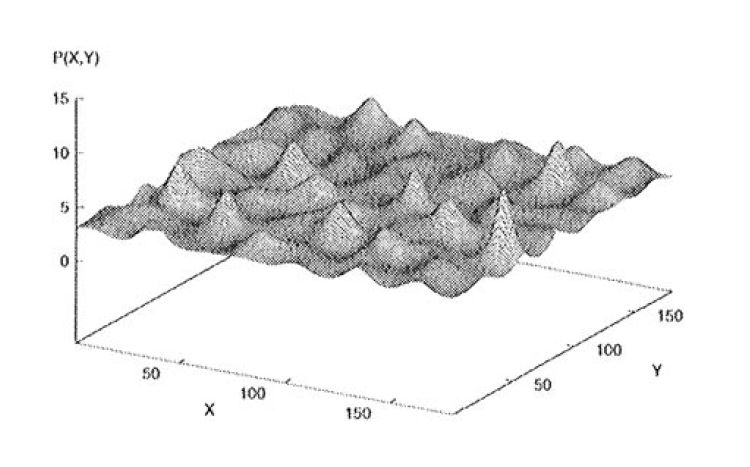
\includegraphics[height=7cm]{fig/cap02/distrubucionPilaresTermitas.JPG}
    \caption{Distribución de los pilares para la construcción de la cámara real de las termitas}
    \label{fig:pillarsTermites}
\end{figure}

\subsection{Modelos basados en agentes}\label{s2_2_2}
Basando sus estudios en la observación de un banco de peces, Aoki parte de dos premisas principales: que la velocidad y dirección de cada individuo son variables estocásticas y se determina otros principios como que el tiempo se cuantificaba como \(\Delta T\) o que el organismo se mueve en dos dimensiones. Adicionalmente, para simplificar el problema limita la interacción entre los individuos al componente direccional y el componente velocidad pasa a determinarse independientemente de los otros elementos del grupo \cite{aoki1982simulation}. 

\begin{figure}[!h]
    \centering
    {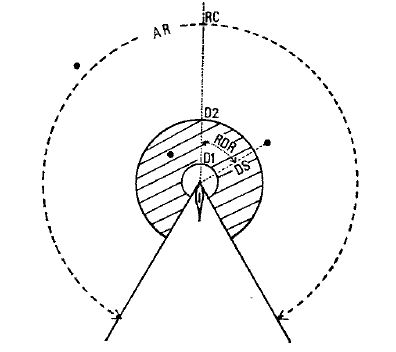
\includegraphics[height=6cm]{fig/cap02/movimientoPecesAoiki.JPG}}
    \caption{Ilustración con los parámetros que influyen en el modelo de Aoki}
    \label{fig:aokiFishInteractions}
\end{figure}\label{fig:aokifish}

Tomando como referencia el esquema representado en la figura \ref{fig:aokifish} y partiendo de las premisas anteriormente expuestas, Aoki define los siguientes modelos matemáticos para definir la distribución de la velocidad:
\begin{equation}\label{eq:velocityDistributionAoki} 
    f(v) = \displaystyle{\frac{A^{K}}{\Gamma (K)}}e^{-Av}v^{K-1}
\end{equation}

\noindent y la probabilidad de alineación en la dirección \(p_{i}(\theta)\):
\begin{equation}\label{eq:directionDistributionAoki}
    p_{i}(\theta)=\sum_{j}W_{j}\frac{1}{S_{j}\sqrt{2\pi}}e^{-(\theta -M_{j})^2/2S_{j}^2} 
\end{equation}


En la ecuación \ref{eq:velocityDistributionAoki} se encuentran  \(\upsilon\) como valor de la velocidad, \textit{K} y \textit{A} como parámetros constantes y mayores que cero y \(\Gamma(K)\) que es una función gamma. En la segunda ecuación (\ref{eq:directionDistributionAoki}) \(W_{j}\) es el factor que pondera la influencia que tiene cada individuo dentro de la distancia \textit{RC}. 

La dirección del movimiento está pues, relacionada con la ubicación y el rumbo de los vecinos. La influencia que ejercen los individuos entre sí se define mediante la ecuación$$ W_{j+1}=RF \cdot W_{j},$$ donde \textit{RF} es una constante entre 0 y 1 definida para cada simulación. Todo esto conlleva a establecer que los individuos pueden tener tres tipos de conductas diferentes dentro del grupo en función de las distancias y las interacciones que tienen: aproximación, sorteo/evitación y orientación paralela.

El modelo descrito anteriormente se programó para realizar los cálculos necesarios, y se ejecutó siguiendo un algoritmo muy bien definido que se muestra en el flujo de figura \ref{fig:flowchartAoki}. Tras ejecutar su modelo numerosas veces cambiando los parámetros de entrada, llegó a la conclusión de que a lo largo de las 2000 iteraciones de cada ejecución, los individuos permanecían en grupo mostrando siempre comportamientos muy similares. 

\begin{figure}[h!]
    \centering
    {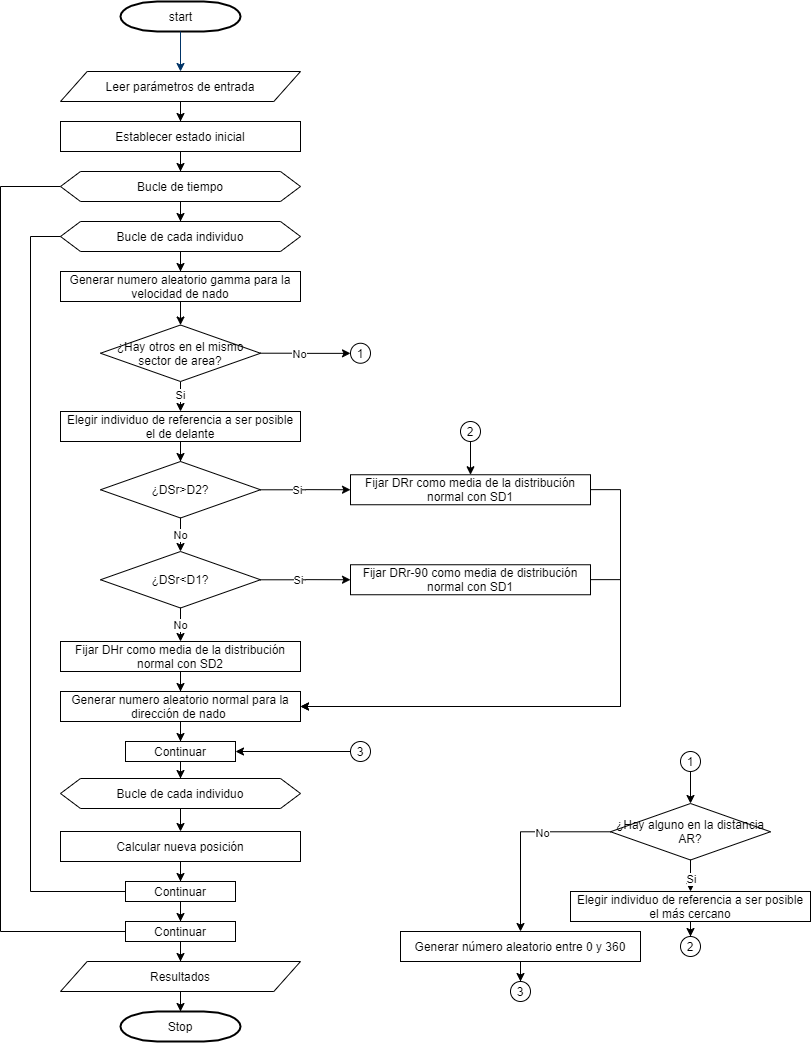
\includegraphics[height=15cm]{fig/cap02/AlgoritmoAoki.png}}
    \caption{Diagrama del flujo del modelo de simulación de Aoki}
    \label{fig:flowchartAoki}
\end{figure}

Estos estudios que inició Aoki, en los que simplifica el modelo con premisas iniciales para poder optimizar las simulaciones, dieron lugar a la exploración desde distintos enfoques de las propiedades de comportamiento con las que están dotadas las especies gregarias como los peces. En estudios posteriores se incluyen la limitación de una pista sensorial para estudiar el cambio de comportamiento \cite{partridge1980sensory,Pitcher963blindfish}, el estudio de las reacciones a objetos estacionarios o móviles \cite{shaw1971optomotor} o el análisis de movimientos individuales y se siguió concluyendo que los movimientos grupales en la unidad podían ocurrir a pesar de carecer cada individuo del conocimiento del movimiento de todo el banco de peces.

Otro estudio, mencionado en un punto anterior, realizado en esta ocasión por Reynolds, se centra en encontrar un modelo óptimo para poder simular el movimiento de una bandada de pájaros en una animación por ordenador \cite{reynolds1987flocks}. Parte de la problemática inicial que tienen otros modelos es la dificultad de simular el movimiento real de animales colectivos ya sean bandada de pájaros, manadas de animales, banco de peces o cualquier grupo dentro del espectro que conocemos y estamos tratando como animales colectivos.

En este estudio, Reynolds se centra en bandadas de pájaros y propone que no es imposible simular el movimiento de un grupo de aves por ordenador, pero se necesita un mejor enfoque para una animación eficiente, robusta y creíble. Para ello el modelo se enfoca desde la suposición de que una bandada es simplemente el resultado de la interacción entre los comportamientos individuales de las aves.

Según el autor, ``el movimiento general parece fluido; tiene un concepto simple, pero es tan visualmente complejo que parece aleatoriamente organizado y, sin embargo, está magníficamente sincronizado'' y es por ello que traslada estos movimientos a un enfoque geométrico.

En un vuelo real, los giros y movimientos ocurren de forma continua y simultánea. Por su parte el vuelo geométrico incremental que propone es una aproximación discreta de esto; pequeños movimientos lineales que modelan una trayectoria curva continua. En términos cartesianos, el eje derecha-izquierda es X, arriba / abajo es Y, y adelante-atrás es Z (ver figura \ref{fig:geometricalFlight}). Adicionalmente a esto, para modelar el vuelo hay que tener en cuenta la gravedad contrarrestada con la flotabilidad del ave por el efecto de las alas.

\begin{figure}[h!]
    \centering
    {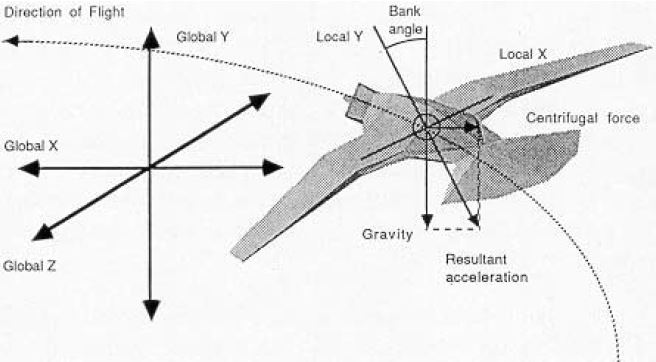
\includegraphics[height=5cm]{fig/cap02/geometricalFlight.JPG}}
    \caption{Geometría del vuelo de Reynolds}
    \label{fig:geometricalFlight}
\end{figure}

Para que se formen las bandadas, cada individuo debe tener comportamientos que permitan la coordinación con los de sus compañeros, que en contra de lo que parece, no son totalmente aleatorios, si no que tienen movimientos comunes.

Un ave puede ser consciente de tres factores: de sí mismo, sus de 5 a 7 de sus vecinos más cercanos \cite{ballerini2008interaction}\footnote{En un principio Reynolds contempla que le influye el comportamiento de sus 2 o 3 vecinos más cercanos, pero es Ballerini et al. quienes demuestran que el número de vecinos está entre 5 y 7.} y el resto de la bandada. Es por esto por lo que una bandada de pájaros no tiene límite de individuos y nunca parece estar sobrecargada ya que la cantidad de factores que un mismo ave tiene que tener en cuenta para mantenerse en la bandada es independiente del número de individuos que la integren. De esta manera, la tarea de volar siempre es igual de simple (o compleja).

Aunque el vuelo en bandada descrito anteriormente resulte aparentemente sencillo, el trabajo requerido para ejecutar el algoritmo en ordenador crece como el cuadrado de la población del rebaño y definitivamente existe un límite superior en el tamaño de las bandadas simuladas implementadas.

\subsection{Modelos de consenso}\label{s2_2_3}

En un contexto en el que cada vez más se tiende a estudiar el comportamiento de los animales para dar respuesta al por qué del movimiento y comportamiento de los animales para poder simularlo e incluso contemplar la posibilidad de imitarlo en el ser humano, no es hasta 1995, cuando Vicsek realiza un estudio bastante simple basado en dos ecuaciones que veremos a continuación. Con tal de imitar la dinámica de movimiento y explicar el consenso de ciertos sistemas, define para sus partículas un impulso inicial con una velocidad absoluta constante y en cada paso de tiempo cada individuo asume la dirección promedio de sus vecinos en un radio establecido \cite{vicsek1995novel}. Basándose en estas asunciones, Vicsek es capaz de demostrar matemáticamente que las simulaciones de movimientos auto-organizados pueden llevarse a cabo.

Para entender matemáticamente este modelo, la posición de cada \(i\)-ésima partícula viene dada por:
\begin{equation}\label{eq:vicsekParticlePosition}
    x_{i}(t+1)=x_{i}(t)+\mathbf{v}_{i}(t)\Delta t
\end{equation}
 donde la velocidad de la partícula $\mathbf{v}_{i}(t+1)$ se construye para tener un valor absoluto $v$ y una dirección dada por el ángulo $\theta (t+1)$ obtenido mediante la expresión: 
 \begin{equation}\label{eq:vicsekParticleDirection}
    \theta (t+1)=\langle\theta (t)\rangle _{r}+\Delta \theta
 \end{equation}
 donde $\langle \theta (t)\rangle _{r}$ es la dirección media de las del grupo que rodea a la partícula $i$ en un radio $r$. También en \ref{eq:vicsekParticleDirection} $\Delta \theta$ es un número aleatorio entre dos valores definidos $[-\mu /2 , \mu /2]$ que representa la perturbación por algún agente externo. 
 
 El resto de su estudio se basa en comprobar el comportamiento que tienen las partículas en base a los dos parámetros básicos, el ruido $\mu$ y la densidad $\rho = N/L^{2}$. Modificando estos valores se da cuenta de que siempre hay consenso entre las partículas en mayor o menor medida. Para densidades y perturbaciones pequeñas, las partículas tienden a formar grupos moviéndose cada uno guardando cierta cohesión. Cuando la densidad y el ruido son muy altos todas las partículas tienden a llevar la misma dirección aunque sea aleatoria. El caso más interesante es cuando la densidad es elevada y la perturbación es baja, en cuyo caso el movimiento se lleva a cabo de manera ordenada a nivel macroscópico. 
 
 Un trabajo de investigación muy interesante que surge a raíz del modelo de Vicsek, es el realizado por Alethea Barbaro y un grupo de científicos y biólogos, en el cual aplica el modelo a la población de capelán islandés para reproducir la ruta de migración durante tres años diferentes, prediciendo con éxito la ruta para 2008 \cite{barbaroModellingSimulations}. El valor de este estudio radica en que en ese año predijeron que llegarían a un lugar donde nunca habían estado. Utilizando los datos de temperatura disponibles y las corrientes aproximadas, pudo reproducir las rutas migratorias observadas de los tres años anteriores \cite{barbaro2009simulations}. Primero se hizo un análisis para identificar la temperatura oceánica y el equilibrio entre la influencia de la interacción entre partículas y la respuesta de las partículas a la temperatura como los parámetros de control más significativos de cara a determinar la ruta de migración.
 
 Otros dos autores que dedican gran parte de su investigación a buscar un modelo de consenso son Felipe cucker y Steve Smale.  Aunque parten de los estudios de Vicsek, la diferencia con éste es que Cucker-Smale (C-S a partir de ahora) calcula la velocidad definiendo primero el vector de posición. Esto es así debido a que en un primer momento observaron que cualquier ``rebaño'' de animales, para el ejemplo me referiré a pájaros, terminan moviéndose a la misma velocidad sea cual sea su posición inicial. \cite{cucker2007emergent}.
 
 En este modelo, la velocidad de cada pájaro ajusta su velocidad añadiéndole una media ponderada de las diferencias de su velocidad con las de las otras aves. 
 
 \begin{equation}\label{eq:CSvelocidad}
     v_{i}(t+1)-v_{i}(t)=\sum_{j=1}^k a_{ij}(v_{j}(t)-v_{i}(t))
 \end{equation}
 
 Aquí, el valor del parámetro $\{a_{ij}\}$ cuantifica la manera en la que los pájaros influyen a los demás, que está relacionada con la distancia a la que se encuentran los pájaros sobre los que se ejerce esta influencia. Este valor también lo calculan mediante la ecuación 
 
 \begin{equation}
     \label{eq:CSaij}
     a_{ij} = \mu(||x_{i}-x_{j}||^2) = \frac{K}{(\sigma^2 + ||x_i-x_j||^2)^\beta}
 \end{equation}
 
 donde por cuestiones de simplicidad, se fijan los valores $K,\sigma>0$ y $\beta \ge 0$. Si se hace la derivada de la ecuación de la velocidad (\ref{eq:CSvelocidad}) obtendremos la función de la aceleración que ya se vio en el Capítulo 1:
 
 \begin{equation}
    \left\lbrace
    \begin{array}{ll}
        \dot{x}_{i}(t)=v_{i}(t) \\
        \dot{v}_{i}(t)= \displaystyle{\frac{1}{N}\sum_{j=1}^{N}\frac{v_{j}(t)-v_{j}(t)}{(1+||x_{j}(t)-x_{j}(t)||^2)^\beta}}
    \end{array}
    \right.
\end{equation}
 
Una de las características de este modelo es que el rebaño siempre llega a consenso sea cual sea su estado inicial, para valores de $\beta \leq 0,5$, correspondiente a una interacción a larga distancia social bastante fuerte. Por el contrario, para valores de $\beta >0.5$ el comportamiento de auto-organización se lleva a cabo bajo unas determinadas condiciones en el estado inicial, como por ejemplo, que el grupo en la posición inicial se encuentre lo más próximo al centro de masa del rebaño.

Para estos casos, si se quiere garantizar el consenso del grupo cuando no se cumplen estas condiciones iniciales, es necesario incluir estrategias de control al modelo, lo cual es el estudio del presente trabajo y se profundizará en el tema más adelante. 

A pesar de la elegancia de los resultados en cuanto a su comportamiento de consenso, la descripción de la dinámica auto-organizada por el modelo C-S sufre de varios inconvenientes que tratan de solucionar Sebastien Motsch y Eitan Tadmor proponiendo un nuevo modelo que no solo tiene en cuenta la distancia entre agentes, sino que también consideran la influencia que ejercen dos agentes entre sí en sus distancias relativas. Como consecuencia, lo que proponen Motsch y Tadmor no implica ninguna dependencia explícita del número de agentes sino que solo se tiene en cuenta su geometría en el espacio \cite{motsch2011new}. Los dos autores proponen en un primer momento el siguiente modelo: 

\begin{equation}
    \label{eq:MTmodel1}
    \left\lbrace
    \begin{array}{lll}
        \dot{x}_{i}(t)= v_{i} \\
        \dot{v}_{i}(t)=\displaystyle{\frac{\alpha}{\sum_{k=1}^{N}\phi_{ik}}\sum_{j=1}^{N}\phi_{ij}(v_{j}-v_{i})} \\ 
        \phi_{ij}=\phi(|x_{j}-x_{i}|)
    \end{array}
    \right.
\end{equation}

En este modelo, $\alpha$ es una constante positiva y $\phi$ es la función de influencia y la característica principal es que la influencia que ejerce el agente ``\textit{j}'' sobre el ``\textit{i}'' está ponderado por la influencia total del grupo $\sum_{k=1}^{N}\phi_{ik}$ ejercida sobre el agente ``\textit{i}''. Si todos los agentes están separados por la misma distancia, entonces este modelo tiende al de C-S, pero a diferencia de éste, la normalización de la interacción por pares entre agentes en términos de influencia relativa tiene como consecuencia la pérdida de simetría.

Por tanto, en agrupaciones grandes, si se pondera correctamente la influencia que ejercen todos los individuos de manera suficientemente lenta en función de la distancia a la que se encuentren, se consigue una cohesión del grupo independientemente de la configuración inicial, evitando de esta manera que sólo influya el comportamiento del vecino más cercano y llegando al consenso de manera mucho más efectiva.

 \subsection{Bertozzi y D'Orsogna}
 El siguiente modelo, propuesto por los autores \citeauthor{d2006self} en \cite{d2006self}, está basado en las- interacciones de atracción-repulsión:

\begin{equation}\label{eq:attractionRepulsion} 
    \left\lbrace
    \begin{array}{ll}
        \dot{x}_{i}(t)=v_{i}(t) \\
        \dot{v}_{i}(t)=\displaystyle{(\alpha - \beta |v_{i}|^{2})v_{i} -\frac{1}{N}\sum_{j\neq 1}\nabla U(|x_{i}-x_{j}|)}
    \end{array}
    \begin{array}{rr}
        (i = 1, ..., N) \\
        (i = 1, ..., N)
    \end{array}
    \right.
\end{equation}

$U$ representa el comportamiento de repulsión o de atracción entre los individuos, y puede definirse de diferentes maneras en función del control que se le quiera otorgar al modelo, por ejemplo, una elección típica es asignarle un valor: 

\begin{equation}\label{eq:potencialU}
    \left\lbrace
    \begin{array}{l}
        U(x) = k(|x|) \\
        k(r) = -C_{A}e^{-r/l_{A}}+-C_{R}e^{-r/l_{R}}
    \end{array}
    \right.
\end{equation}

donde $C_A$, $C_R$ y $l_A$, $l_R$ representan las fuerzas y longitudes típicas de atracción y repulsión respectivamente. Al depender de estos 4 parámetros, las posibilidades de comportamiento son muy diferentes, en función de los valores que se les asignen, por ejemplo, para valores $C_R = 50$, $l_R = 2$, $C_A = 20$, $l_A = 100$, $\alpha = 0.07$ y $\beta = 0.05$, encontramos que los individuos se organizan en una especie de remolino como en \ref{fig:remolino}. Sin embargo si a estos parámetros les asignamos los valores $C_R = 50$, $l_R = 20$, $C_A = 100$, $l_A = 100$, $\alpha = 0.15$ y $\beta = 0.05$ el resultado es que los individuos igualmente terminan formando un remolino, pero algunos de ellos en dirección a las agujas del reloj, mientras que otros, en sentido contrario. 

\begin{figure}[!ht]
\centering
    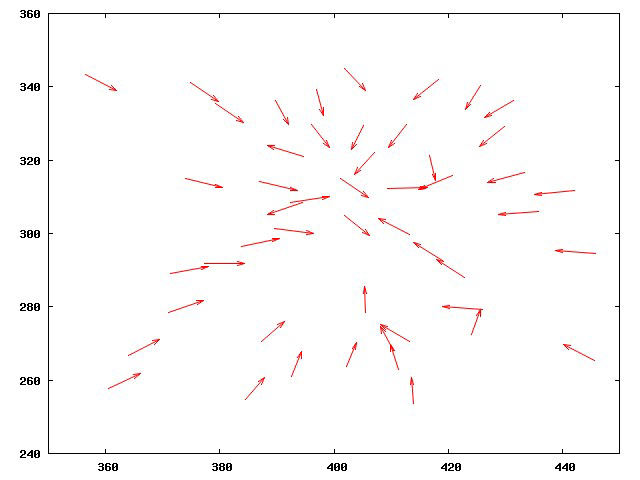
\includegraphics[scale=0.3]{fig/cap02/atraccionRepulsion/11.png}
    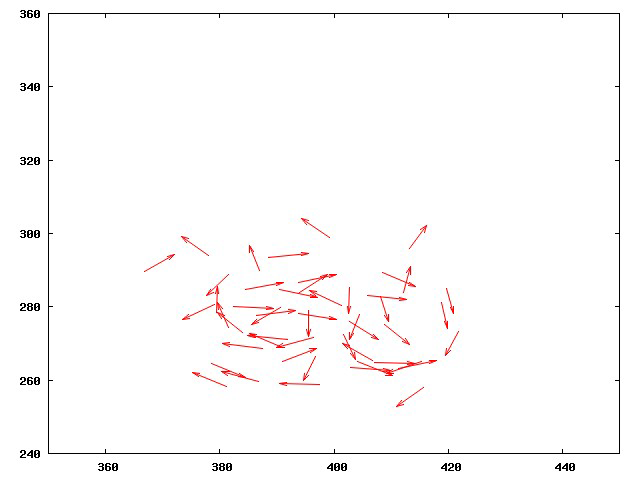
\includegraphics[scale=0.3]{fig/cap02/atraccionRepulsion/12.png}
    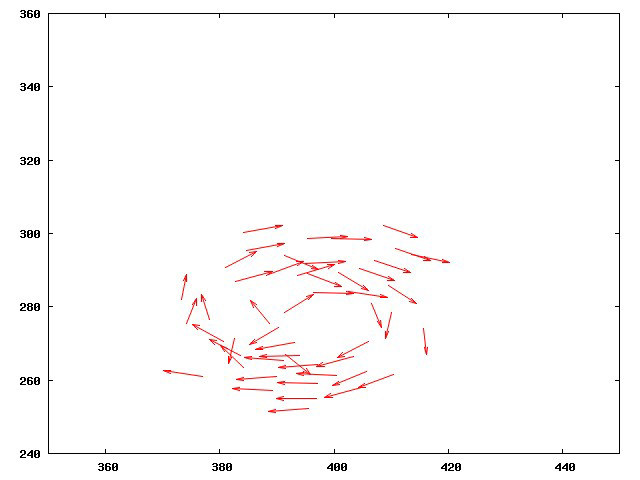
\includegraphics[scale=0.3]{fig/cap02/atraccionRepulsion/13.png}
    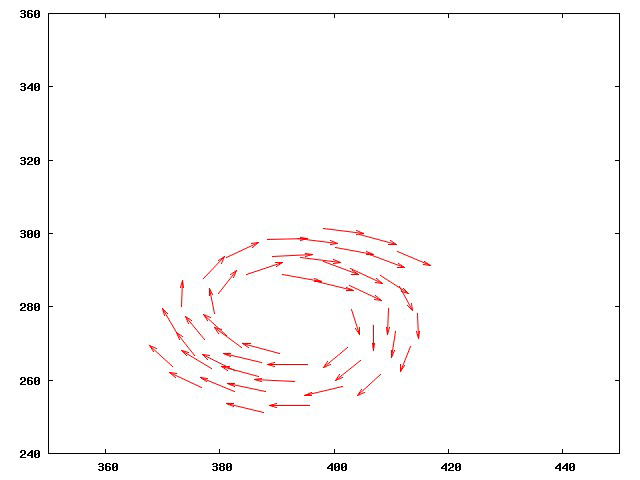
\includegraphics[scale=0.3]{fig/cap02/atraccionRepulsion/14.png}
\caption{Hormiga tejedora (\textit{Oecophylla})}
\label{fig:remolino}
\end{figure}

Por tanto concluyen en este estudio que el comportamiento del grupo puede controlarse exclusivamente con los parámetros $\alpha$, $\beta$, $C_A$, $C_R$ y $l_A$, $l_R$.